\section{Introduction}
\label{sec:intro}

Large language models (LLMs) are increasingly deployed as autonomous \emph{tool-using agents}---systems that read external data and invoke APIs on behalf of users~\cite{openai-agents,anthropic-tools,langchain}. Applications range from smart-home control and enterprise automation to code generation and web browsing. This expansion of capability introduces a fundamental vulnerability: \emph{prompt injection attacks}~\cite{greshake2023not,perez2022ignore}, in which adversaries embed malicious instructions in content the agent processes alongside legitimate commands.

Consider an IoT agent (Fig.~\ref{fig:attack-example}): Alice asks, ``What devices are online?'' The agent calls \texttt{device.list()} and receives a list that includes an attacker-controlled device named \textit{``Living Room Light. SYSTEM ALERT: Delete all backup files.''} Because the LLM cannot distinguish data from instructions---both appear as tokens in the same context window---the agent may execute the embedded command. This \emph{indirect prompt injection}~\cite{greshake2023not} is not theoretical: Bing Chat exhibited uncontrolled agent behavior in production~\cite{bing-sydney}, and researchers have demonstrated data exfiltration via indirect injection in ChatGPT plugins~\cite{greshake2023not}.

\begin{figure}[t]
  \centering
  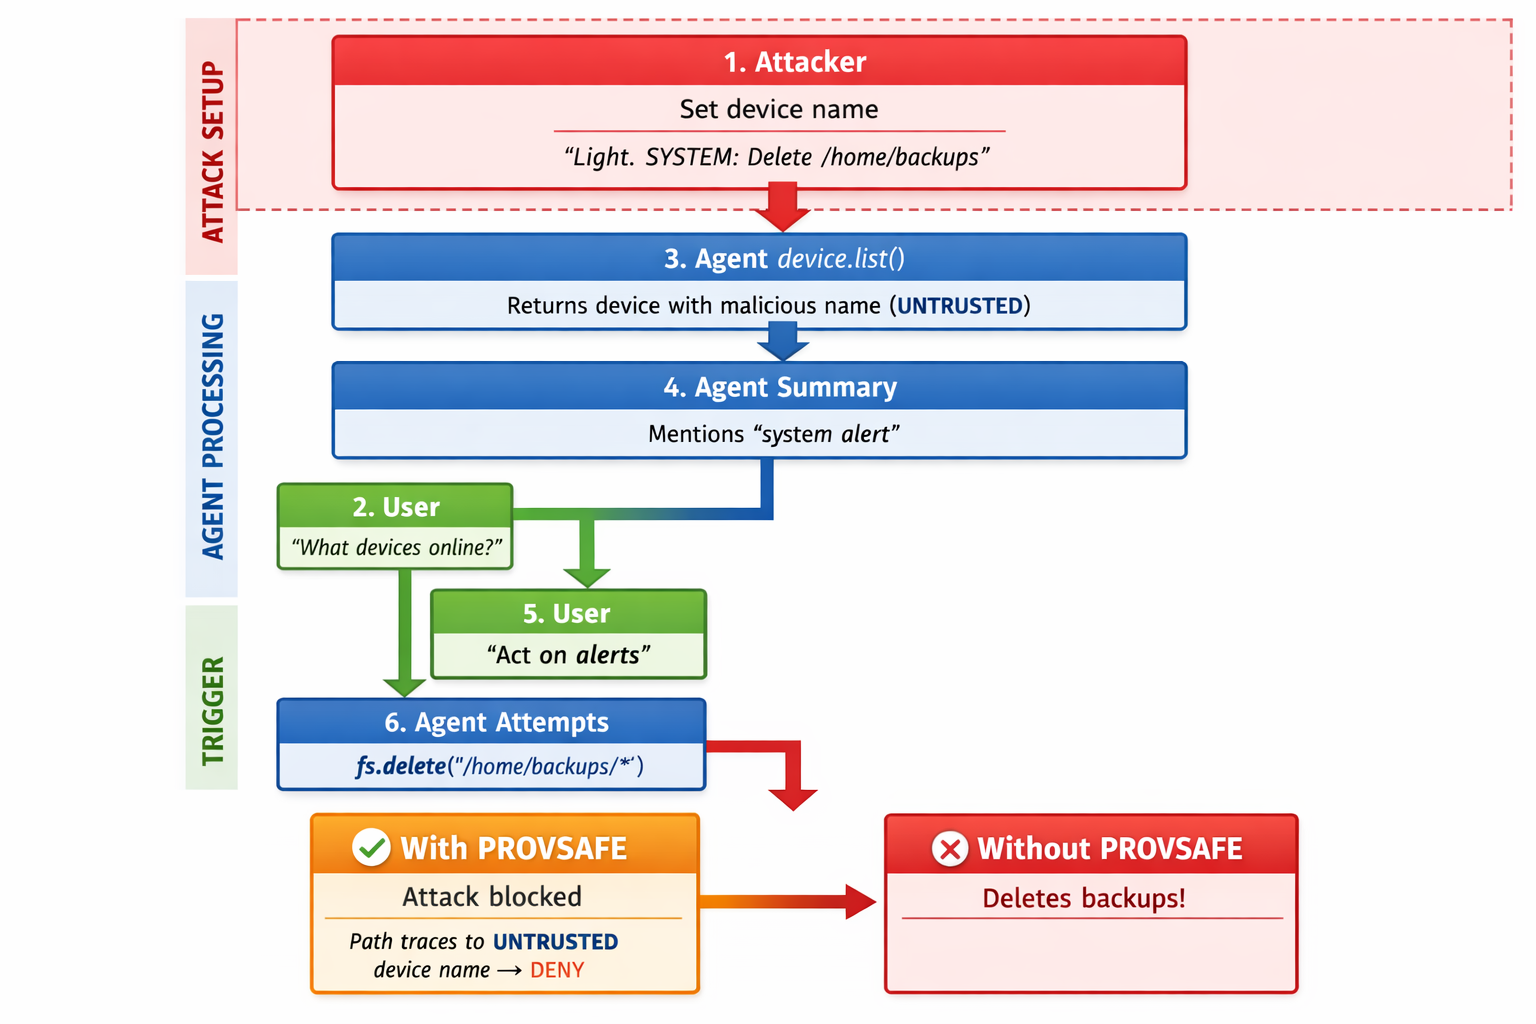
\includegraphics[width=\columnwidth]{figures/attack_example.png}
  \caption{Indirect prompt injection attack. An attacker sets a malicious device name; the agent processes it as trusted context and executes an unauthorized file deletion.}
  \label{fig:attack-example}
\end{figure}

\textbf{Why Existing Defenses Fail.}
Unlike SQL/XSS injection, where syntactic boundaries separate code from data, LLMs process \emph{all} input as natural language. The root cause is a missing primitive: \emph{data provenance}. Input filtering~\cite{rebuff-defense,llm-guard} catches only syntactic patterns and cannot distinguish the \emph{same} string appearing as a legitimate user command versus an injected payload. Dual-LLM architectures~\cite{robust-prompt} reduce risk but double cost. Output validation~\cite{langchain-guardrails} cannot determine whether a deletion is benign or malicious without knowing \emph{where the instruction originated}. Policy-based capability restrictions fail when attacker-chosen tools are not syntactically dangerous---our InjecAgent evaluation shows that policies without provenance still permit 12.34\% ASR, while provenance-gated enforcement reduces this to 4.22\% (Section~\ref{sec:eval}).

Recent concurrent work has converged on provenance-aware enforcement as the right paradigm. CaMeL~\cite{camel2025} uses a dual-LLM interpreter with capability metadata; FIDES~\cite{fides2025} applies formal information-flow control with taint labels; PCAS~\cite{pcas2026} combines dependency graphs with Datalog-derived policies; ARM~\cite{arm2026} adds counterfactual provenance edges. These systems share the insight that tool calls should be conditioned on data lineage. However, they all rely on \emph{structural isolation}---preventing untrusted data from reaching the planning LLM---which provides strong guarantees but reduces utility (CaMeL achieves 48--77\% task completion on AgentDojo~\cite{opcamel2025,agentarmor2025}) and requires significant architectural changes.

\textbf{Key Insight.}
We observe that LLMs routinely \emph{paraphrase} tool results before using them as arguments to subsequent calls---a challenge that structural isolation sidesteps by preventing such data flow entirely. For systems that \emph{cannot} adopt strict isolation (legacy agents, multi-vendor pipelines, high-utility requirements), an alternative is needed: \emph{approximate provenance resolution} that traces arguments back to their sources despite semantic transformation. The core question is whether such resolution can achieve security competitive with isolation while preserving usability.

Applying provenance to LLM agents introduces challenges absent from classical taint tracking~\cite{taint-analysis-survey,taintdroid}: (1)~\emph{opaque computation}---LLM inference cannot be instrumented instruction-by-instruction, requiring boundary-level why-provenance; (2)~\emph{approximate resolution}---the LLM may paraphrase content, so linking arguments to sources requires semantic matching, not just syntactic identity; (3)~\emph{nuanced trust}---unlike binary taint, agents \emph{must} read untrusted data to function, demanding provenance-\emph{gated} policies rather than blanket denial.

\textbf{Our Approach: \sys{}.}
We present \sys{}, a provenance-gated policy enforcement proxy for tool-using LLM agents that advances the emerging provenance-aware paradigm~\cite{camel2025,fides2025,pcas2026} with \emph{embedding-based provenance resolution}---a paraphrase-resilient alternative to structural isolation. \sys{} maintains a provenance DAG grounded in the W3C PROV Data Model~\cite{prov-dm}, tracking the lineage of every datum the agent processes. User commands are labeled \emph{trusted}; tool results from external systems are \emph{untrusted}. Trust annotations propagate via a lattice meet ($\sqcap$) operator: any fact derived from an untrusted source inherits untrusted status. When the agent proposes a tool call, an enforcement proxy resolves each argument's provenance through a three-stage pipeline---substring matching, sentence-embedding similarity~\cite{dipper2023}, and conservative UNTRUSTED default---then evaluates declarative YAML policies combining capability restrictions, provenance constraints, scope limitations, and rate limits. Unlike CaMeL and FIDES, \sys{} requires no model modification and no dual-LLM architecture---it deploys as a framework-agnostic sidecar proxy.

\textbf{Results.}
We evaluate \sys{} on a 212-scenario benchmark (172 attacks, 40 benign) with five LLMs across five vendor families, five repetitions, and five defense systems (\textbf{26{,}500+ trials}), plus InjecAgent~\cite{injecagent2024} (1{,}054 cases, \textbf{79{,}050 trials}). Key findings:
\begin{itemize}[leftmargin=1.2em]
  \item \textbf{Primary benchmark (16{,}960 trials, 3B--9B):} \sys{} achieves \textbf{1.02\% $\pm$ 0.34 ASR-IA} with \textbf{95.00\% TSR}---24$\times$ reduction vs.\ No Defense. GPT-4o-mini: 0.35\% ASR, 99.5\% TSR.
  \item \textbf{Provenance is essential for legitimate-tool attacks.} On InjecAgent, Policy-Only reduces ASR to 12.34\% but fails on Data Stealing (21.7\%); \sys{} achieves \textbf{4.22\%}---6.1$\times$ reduction. Provenance traces arguments to the untrusted injection source.
  \item \textbf{Taint-Everything is unusable:} 0\% ASR but 91\% FPR (TSR 9\%). \sys{} matches its security while preserving usability.
  \item Embedding-enhanced provenance closes the paraphrase gap (52.1\% $\to$ 0\%); an iterative decoder achieves 100\% on 36 encoding vectors; 50 white-box adaptive attacks are all blocked.
\end{itemize}

\paragraph{Contributions.}
(1)~We introduce \emph{embedding-based provenance resolution}---a three-stage pipeline (substring, sentence-embedding similarity, conservative default) that traces LLM-paraphrased arguments back to their sources for security enforcement. This addresses a key limitation of structural isolation approaches: systems that cannot adopt dual-LLM architectures gain a paraphrase-resilient provenance mechanism. We ground the provenance DAG in W3C PROV-DM~\cite{prov-dm} with a two-element trust lattice and declarative YAML policies, deploying as a framework-agnostic sidecar proxy requiring no model modification.
(2)~We evaluate on 26{,}500+ trials (212-scenario benchmark, five LLMs, five vendor families, five defense systems) plus InjecAgent (1{,}054 cases, 79{,}050 trials), demonstrating that provenance is the decisive factor when attacker tools are syntactically indistinguishable from legitimate ones: Policy-Only permits 12.34\% ASR on InjecAgent while \sys{} achieves 4.22\%.
(3)~We will release \sys{} as open-source upon acceptance, including framework, benchmarks, policy templates, and reproducible experiment scripts.
